\documentclass[a4paper,11pt]{article}

\usepackage[utf8]{inputenc}
\usepackage[T1]{fontenc}
\usepackage[english]{babel}
\usepackage{graphicx}
\usepackage{amsmath,amssymb,amsthm,amsopn}
\usepackage{mathrsfs}
\usepackage{graphicx}
\usepackage{array}
\usepackage{makecell}


\usepackage{hyperref}
\hypersetup{
    colorlinks=true,
    linkcolor=blue,
    citecolor=red,
}

%\usepackage[top=1cm,bottom=1cm]{geometry}
%\usepackage{listings}
%\usepackage{xcolor}

\usepackage{tikz}

% Tikz style

\tikzset{round/.style={circle, draw=black, very thick, scale = 0.7}}
\tikzset{arrow/.style={->, >=latex}}
\tikzset{dashed-arrow/.style={->, >=latex, dashed}}

\newtheoremstyle{break}%
{}{}%
{\itshape}{}%
{\bfseries}{}%  % Note that final punctuation is omitted.
{\newline}{}

\newtheoremstyle{sc}%
{}{}%
{}{}%
{\scshape}{}%  % Note that final punctuation is omitted.
{\newline}{}

\theoremstyle{break}
\newtheorem{thm}{Theorem}[section]
\newtheorem{lm}[thm]{Lemma}
\newtheorem{prop}[thm]{Proposition}
\newtheorem{cor}[thm]{Corollary}

\theoremstyle{sc}
\newtheorem{exo}{Exercice}

\theoremstyle{definition}
\newtheorem{defi}[thm]{Definition}
\newtheorem{ex}[thm]{Example}

\theoremstyle{remark}
\newtheorem{rem}[thm]{Remark}

% Math Operators

\DeclareMathOperator{\Card}{Card}
\DeclareMathOperator{\Gal}{Gal}
\DeclareMathOperator{\Id}{Id}
\DeclareMathOperator{\Img}{Im}
\DeclareMathOperator{\Ker}{Ker}
\DeclareMathOperator{\Minpoly}{Minpoly}
\DeclareMathOperator{\Mod}{mod}
\DeclareMathOperator{\Ord}{Ord}
\DeclareMathOperator{\ppcm}{ppcm}
\DeclareMathOperator{\Tr}{Tr}
\DeclareMathOperator{\Vect}{Vect}

% Shortcuts

\newcommand{\dE}{\partial(E)}
\newcommand{\dF}{\partial(F)}
\newcommand{\dG}{\partial(G)}
\newcommand{\diff}{\mathop{}\!\mathrm{d}}
\newcommand{\eg}{\emph{e.g. }}
\newcommand{\emb}{\hookrightarrow}
\newcommand{\embed}[2]{\phi_{#1\hookrightarrow#2}}
\newcommand{\ent}[2]{[\![#1,#2]\!]}
\newcommand{\ie}{\emph{i.e. }}
\newcommand{\ps}[2]{\left\langle#1,#2\right\rangle}





% opening
\title{Examples of compatibility}
\author{}



\begin{document}

\maketitle

%\begin{abstract}

%\end{abstract}

%\tableofcontents

%\clearpage

In this document, we investigate compatibility questions in concrete examples.
We set a prime finite field $k=\mathbb{F}_p$ and we look at the tower of
$\ell$-adic extensions 
\[
  \mathbb{F}_p \emb \mathbb{F}_{p^\ell} \emb \mathbb{F}_{p^{\ell^2}}\emb \cdots
\]
wondering if we can compute compatible embeddings between the fields in this
tower. By compatibility, we mean that we want to find solutions $\alpha_i$ of
Hilbert 90 in $\mathbb{F}_{p^{\ell^i}}\otimes\mathbb{F}_p(\zeta_i)$, where
$\zeta_i$ is a primitive $\ell^i$-th root of unity, and such that for all $j<i$, we
have that 
\[
  \alpha_i^{\ell^{i-j}}=\alpha_j.
\]
We see in Section~\ref{sec:p5l2} that it seems to be possible when the roots
$\zeta_i$ are in the prime field $\mathbb{F}_p$. But Section~\ref{sec:p3l2}
shows that this does not hold in the general case.

\section{Case $p=5$ and $\ell=2$}
\label{sec:p5l2}

Here we have $k=\mathbb{F}_5$,
we choose
\[
  \mathbb{F}_{5^2}\cong\mathbb{F}_5[X]/(X^2-2)\cong\mathbb{F}_5(t)
\]
where
$t=\overline X$ is such that $t^2=2$. And we choose 
\[
  \mathbb{F}_{5^4}\cong
\mathbb{F}_{5^2}[Y]/(Y^2-t)\cong \mathbb{F}_{5^2}(u)
\]
where $u=\overline
Y$ is such that $u^2 = t$. We have exactly one primitive square root of
unity in $\mathbb{F}_5$ that is $\zeta_1 = -1$ and two $4$-th
root of unity $\zeta_2=\pm 2$. The situation is described in
Figure~\ref{fig:p5l2}.

\begin{figure}
  \centering
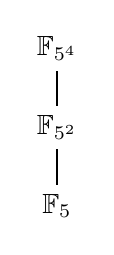
\begin{tikzpicture}
  \node (1) at (0,0) {$\mathbb{F}_{5}$};
  \node (2) at (0,1) {$\mathbb{F}_{5^2}$};
  \node (4) at (0,2) {$\mathbb{F}_{5^4}$};

  \draw (1) -- (2);
  \draw (2) -- (4);
\end{tikzpicture}
\phantom{and}
\begin{tikzpicture}
  \node (1) at (0,0) {$1$};
  \node (2) at (0,1) {$-1$};
  \node (4a) at (-.5,2) {$2$};
  \node (4b) at (.5,2) {$-2$};

  \draw (1) -- (2);
  \draw (2) -- (4a);
  \draw (2) -- (4b);
\end{tikzpicture}
  \caption{Tower of extension with $p=5$ and $\ell=2$, and the associated roots.}
  \label{fig:p5l2}
\end{figure}

Assume we have computed a solution $\alpha_1$ of Hilbert 90 in
$\mathbb{F}_{5^2}$ for $\zeta_1=-1$, for example $\alpha_1=t$. Indeed, we have 
\[
  t^5 = t^4\times t = -t
\]
since $t^2=2$. We now wonder if we can compute a solution $\alpha_2$ of Hilbert
90 in $\mathbb{F}_{5^4}$ for $\zeta_2$ such that $\alpha_2^2=\alpha_1$. The
answer depends on the choice of the root $\zeta_2$ we take. Let us start with
$\zeta_2 = 2$. We want to solve
\[
  \sigma(\alpha) = 2\alpha,
\]
and a solution is given by 
\[
  \alpha = u,
\]
since $u^2 = t$ and $t^2 = 2$. The other nonzero solutions are $2u$, $3u$ and
$4u$. We have $u^2 = t$, so we are able to choose $\alpha_2$ such that
$\alpha_2^2 = \alpha_1$. Now if we work with the root $\zeta_2=-2$, we now want
to solve
\[
  \sigma(\alpha) = -2\alpha,
\]
and a solution is given by
\[
  \alpha = ut
\]
since $(ut)^2 = 2t$ and $(2t)^2 = -2$. The other nonzero solutions are $2ut$, $3ut$ and
$4ut$. Now we have $(ut)^2 = 2t$ and $2$ is not a square in $\mathbb{F}_5$ so we
are not able to choose a solution $\alpha_2$ of the Hilbert 90 problem for the
root $\zeta_2=-2$ such that $\alpha_2^2=\alpha_1$.

If we choose another solution $\alpha_1$ of the Hilbert 90 problem in
$\mathbb{F}_{5^2}$, then there is still exactly one root $\zeta_2$ that allows to find a
solution $\alpha_2$ with $\alpha_2^2=\alpha_1$. The hope was that, in general,
every choice of solution $\alpha_1$ is compatible with a root $\zeta_2$, where by
compatible we mean that there is a solution $\alpha_2$ with
$\alpha_2^2=\alpha_1$. This is not true, as shows Section~\ref{sec:p3l2}.

\section{Case $p=3$ and $\ell=2$}
\label{sec:p3l2}

Here we have $k=\mathbb{F}_3$,
we choose
\[
  \mathbb{F}_{3^2}\cong\mathbb{F}_3[X]/(X^2+1)\cong\mathbb{F}_3(t)
\]
where
$t=\overline X$ is such that $t^2=-1$. And we choose 
\[
  \mathbb{F}_{3^4}\cong
\mathbb{F}_{3^2}[Y]/(Y^2-(t+1))\cong \mathbb{F}_{3^2}(u)
\]
where $u=\overline
Y$ is such that $u^2 = t+1$. We have exactly one primitive square root of
unity in $\mathbb{F}_3$ that is $\zeta_1 = -1$ and we do not have any primitive $4$-th
root of unity $\zeta_2$ in $\mathbb{F}_3$, but we have two of these roots in
$\mathbb{F}_3(\zeta_2)\cong \mathbb{F}_{3^2}$: $\pm t$. The situation is
summarised in Figure~\ref{fig:p3l2}.

\begin{figure}
  \centering
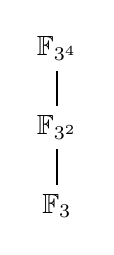
\begin{tikzpicture}
  \node (1) at (0,0) {$\mathbb{F}_{3}$};
  \node (2) at (0,1) {$\mathbb{F}_{3^2}$};
  \node (4) at (0,2) {$\mathbb{F}_{3^4}$};

  \draw (1) -- (2);
  \draw (2) -- (4);
\end{tikzpicture}
\phantom{and}
\begin{tikzpicture}
  \node (1) at (0,0) {$1$};
  \node (2) at (0,1) {$-1$};
  \node (4a) at (-.5,2) {$t$};
  \node (4b) at (.5,2) {$-t$};

  \draw (1) -- (2);
  \draw (2) -- (4a);
  \draw (2) -- (4b);
\end{tikzpicture}
  \caption{Tower of extension with $p=3$ and $\ell=2$, and the associated roots.}
  \label{fig:p3l2}
\end{figure}



Assume we have computed a solution $\alpha_1$ of Hilbert 90 in $\mathbb{F}_{3^2}$ for
$\zeta_1$, for example $\alpha_1=t$. We indeed have
\[
  t^3 = t^2\times t=-1\times t.
\]
We now wonder if we can compute a solution $\alpha_2$ of Hilbert 90 in
$\mathbb{F}_{3^4}\otimes\mathbb{F}_{3^2}$ for $1\otimes\zeta_2$ such
that $\alpha_2^2=\alpha_1$. Assume we choose $\zeta_2=t$, we want to solve
\[
  (\sigma\otimes\Id)(\alpha) = (1\otimes t)\alpha,
\]
and a solution is given by 
\[
  \alpha = u\otimes1-u^3\otimes t.
\]
Indeed, we have:
\begin{align*}
  (\sigma\otimes\Id)(\alpha) &= u^3\otimes1-u^9\otimes t \\
  &= u^3\otimes 1+u\otimes t \;\;(u^8 = -1)\\
  &= (1\otimes t)(u\otimes1-u^3\otimes t) \\
  &= (1\otimes t)\alpha,
\end{align*}
and the theory tells us that the other solutions are given by $(1\otimes
x)\alpha$ for $x\in\mathbb{F}_{3^2}$. If we compute $\alpha^2$, we get:
\begin{align*}
\alpha^2 &= (u\otimes1-u^3\otimes t)^2 \\
&= u^2\otimes 1 + u^4\otimes t + u^6\otimes t^2 \\
&= -t\otimes 1 - t\otimes t\;\;(u^2=t+1, u^4=-t, u^6=1-t)\\
&= -t\otimes (t+1) \\
&= (1\otimes (2t+2))\cdot(t\otimes 1),
\end{align*}
so we have $\alpha^2=c\alpha_1$ with $c=1\otimes (2t+2)$ and $2t+2$ is not a
square in $\mathbb{F}_{3^2}$, so this is impossible to choose a solution
$\alpha_2$ such that $\alpha_2^2=\alpha_1$.

Now assume we choose $\zeta_2=2t$. In that case we want to solve
\[
  (\sigma\otimes\Id)(\alpha) = (1\otimes 2t)\alpha,
\]
and a solution is given by 
\[
  \alpha = u\otimes1 + u^3\otimes t.
\]
Indeed, we have
\begin{align*}
  (\sigma\otimes\Id)(\alpha) &= u^3\otimes1-u\otimes t \\
  &= (1\otimes 2t)\alpha,
\end{align*}
and we compute
\[
  \alpha^2 = (1\otimes (t+1))\alpha_1.
\]
In that case, we get $c=1\otimes(t+1)$, but $t+1$ is not a square in
$\mathbb{F}_{3^2}$ either. So, with the choice of $\alpha_1=t$, there is no root
$\zeta_2$ such that we can find a solution $\alpha_2$ with
$\alpha_2^2=\alpha_1$. Since the set of solutions of Hilbert 90 in
$\mathbb{F}_{3^2}$ for the root $\zeta_1=-1$ is a $\mathbb{F}_3$ vector space of
dimension one, there is only one other nonzero solution that is the opposite of
the first one: $\alpha_1= -t$. Therefore, the same calculations would show that
we get the coefficient $c=1\otimes (t+1)$ with the root $\zeta_2=t$ and
$c=1\otimes(2t+2)$ with the root $\zeta_2=2t$. As a conclusion, there is no
solution $\alpha_1$ of the Hilbert 90 problem in $\mathbb{F}_{3^2}$ that allows to
find a compatible solution $\alpha_2$ in
$\mathbb{F}_{3^4}\otimes\mathbb{F}_{3^2}$.

\section{An idea of what is happening}
Let $\mathbb{F}_{p^m}\cong K_1\emb K_2\cong \mathbb{F}_{p^n}$ be an extension,
and $d=n/m$ the degree of the extention. Suppose we have an element $\alpha_1$ in $K_1\otimes k(\zeta_1)$ solution of
the Hilbert 90 problem for $1\otimes\zeta_1$, where
$k=\mathbb{F}_p$ and $\zeta_1$ is a $m$-th primitive root of unity. Now assume
we have computed a solution $\alpha_2$ of Hilbert 90 in $K_2\otimes k(\zeta_2)$ for
$1\otimes\zeta_2$, where $\zeta_2$ is a $n$-th primitive root of unity such that
$\zeta_2^d=\zeta_1$. Then we have 
\begin{align*}
  (\sigma\otimes\Id)(\alpha_2^d) &= (\sigma\otimes\Id)(\alpha_2)^d \\
  &= (1\otimes\zeta_2)^d\alpha_2^d \\
  &= (1\otimes\zeta_1)\alpha_2^d
\end{align*}
so $\alpha_2^d$ is a solution of the Hilbert 90 problem for $1\otimes\zeta_1$ in
$K_2\otimes k(\zeta_2)$ and moreover, we have that
\begin{align*}
  (\sigma\otimes\Id)^m(\alpha_2^d) &= (1\otimes\zeta_1)^m\alpha_2^d \\
  &= \alpha_2^d.
\end{align*}
The element $\alpha_2^d$ is fixed by $\sigma^m\otimes\Id$,
so $\alpha_2^d$ is in fact in $K_1\otimes k(\zeta_2)$, but is not in
$K_1\otimes k(\zeta_1)$ in general, as we can see in Section~\ref{sec:p3l2}.

\end{document}
